\documentclass{article}
\usepackage[letterpaper,top=2cm,bottom=2cm,left=3cm,right=3cm,marginparwidth=1.75cm]{geometry}
\usepackage{tikz}
\usetikzlibrary{automata, arrows.meta, positioning}
\usepackage{amsmath}
\usepackage{graphicx}
\usepackage[colorlinks=true, allcolors=blue]{hyperref}
\usepackage[spanish]{babel}
\usepackage[style=apa]{biblatex}
 \usepackage{listings}


\begin{document}
\begin{titlepage}
\centering
\begin{figure}
\centering
 
\vspace{5cm}
\centering
\begin{Huge}
\begin{center}


\includegraphics[scale=2]{imagenes/Bind.png} 

\vspace{2cm}
\end{center}

\end{Huge}
\end{figure}


 {\scshape\Large Práctica Servidor DNS Maestro\par}
\vspace{8cm}

{\Large Ignacio Fernández Contreras\par}
{\Large 4º Informática A\par}
\vspace{0.5cm}
{\large E.T.S. Informática}
\vfill

\end{titlepage}
\clearpage\hbox{}\thispagestyle{empty}\newpage

%-------------------------- EJERCICIO 1 ----------------------

 \newpage
\section{Enunciado}
\begin{flushleft}
El ayuntamiento de Fuengirola quiere montar una red de equipos para monitorizar las casetas de  la feria de Octubre 2023. Para ello nos ha pedido que instalemos un servidor DNS privado con un nuevo dominio de zona llamado “feria.fuengirola”. Todos los equipos de la red (uno por caseta) pertenecerán a dicho dominio que funcionará únicamente de forma privada en la red interna, no en Internet.
El nombre completo de los equipos terminará con el dominio “feria.fuengirola”, por ejemplo: “caseta5.feria.fuengirola”. Lo ideal en una situación así es disponer de un servidor DNS que sea maestro de nuestro dominio, es decir, maestro del dominio interno “feria.fuengirola”.
El servidor DNS maestro para el nuevo dominio interno “feria.fuengirola” será capaz de resolver peticiones internas de nombres de este dominio, tanto de forma directa como de forma inversa, es decir, si recibe una consulta acerca de quién es “caseta.feria.fuengirola” deberá devolver su IP (por ejemplo, 10.0.2.15). Si la consulta es una consulta DNS inversa acerca de quién es 10.0.2.15, deberá responder “caseta5.feria.fuengirola”.

Archivo de zona de búsqueda directa

Supongamos que en la red local tenemos 8 casetas con 1 PCs por caseta con IPs que van desde 10.0.2.15, o su correspondiente IP en su máquina, hasta la IP 22 y cuyos nombres van desde caseta1 hasta caseta8. Luego también se dispone de un servidor web (desplegado en el PC de la caseta2) y un servidor de correo electrónico que además es servidor DNS (desplegado en el PC de la caseta 1). Además, para diferenciar estos hosts de forma fácil se dispondrá de dos alias: “juventud.feria.fuengirola” para el PC de la caseta2 que se corresponde con la caseta de la juventud, y “boliches.feria.fuengirola” para el PC de la caseta1 que se corresponde con la caseta llamada Boliches.
\end{flushleft}

 \section{Resolución}
 
 \textbf{Actualización del sistema e instalación de bind}
 \lstset{language=C, breaklines=true, basicstyle=\footnotesize}
\begin{lstlisting}[frame=single]
sudo apt update
sudo apt install bind
\end{lstlisting}
 
Una vez instalado, tendremos el path: /etc/bind\\

\begin{center}
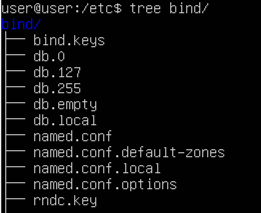
\includegraphics[scale=0.8]{imagenes/img1.png} 
\end{center}


\textbf{Configuración del archivo de zona:}
BIND utiliza archivos de zona para definir la información de los registros DNS.Los archivos de zona se almacenan generalmente en el directorio /etc/bind/zones/
 \lstset{language=C, breaklines=true, basicstyle=\footnotesize}
\begin{lstlisting}[frame=single]
zone "feria.fuengirola" {
	type master;
	file "/etc/bind/zones/feria.fuengirola.zone";
};
\end{lstlisting}
 
 \textbf{Verificación de la configuración:}
  \lstset{language=C, breaklines=true, basicstyle=\footnotesize}
\begin{lstlisting}[frame=single]
sudo named-checkconf
\end{lstlisting}

\textbf{Configuración de las zones:}

\textbf{etc/bind/zones/feria.fuengirola.zone}

  \lstset{language=C, breaklines=true, basicstyle=\footnotesize}
\begin{lstlisting}[frame=single]
$TTL 86400
@	IN	SOA	feria.fuengirola.admin.feria.fuengirola.	(
				2023102101; Serial
				3600;	Refresh
				1800;	Retry
				604800;	Expire
				86400;	Minimum TTL
			)

@	IN	NS	feria.fuengirola.
@	IN	A	10.0.2.1;	
caseta2	IN	A	10.0.2.16
caseta1	IN	A	10.0.2.15

; Alias
juventud	IN	CNAME	caseta2.feria.fuengirola.
boliches	IN	CNAME	caseta1.feria.fuengirola.
\end{lstlisting}



\textbf{etc/bind/zones/10.0.2.zone}

  \lstset{language=C, breaklines=true, basicstyle=\footnotesize}
\begin{lstlisting}[frame=single]
$TTL 86400
@	IN	SOA	feria.fuengirola.admin.feria.fuengirola.	(
			2023102101; Serial
			3600;	Refresh
			1800;	Retry
			604800;	Expire
			86400;	Minimum TTL
		)

@	IN	NS	feria.fuengirola.
15	IN	PTR	boliches.feria.fuengirola.
16	IN	PTR	juventud.feria.fuengirola.
\end{lstlisting}


\textbf{Iniciamos el servidor bind:}

  \lstset{language=C, breaklines=true, basicstyle=\footnotesize}
\begin{lstlisting}[frame=single]
sudo systemctl start bind9
\end{lstlisting}

\textbf{Permitimos el tráfico entrante en un puerto específico:}
\begin{lstlisting}[frame=single]
sudo ufw allow bind9
\end{lstlisting}


\textbf{Quedará un tree:}
\begin{center}
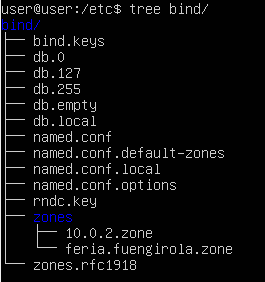
\includegraphics[scale=0.7]{imagenes/img2.png} 
\end{center}


\end{document}